% !TEX program = xelatex
% XeLaTeX source for the 5 x 8 inch edition.
\documentclass[10pt,twoside,openany]{book}

\usepackage{geometry}
\geometry{
  paperwidth=5in,
  paperheight=8in,
  top=0.7in,
  bottom=0.7in,
  inner=0.5in,
  outer=0.5in,
  headheight=10pt,
  headsep=20pt,
  footskip=25.2pt
}
\addtolength{\textheight}{-12pt}

\usepackage{fontspec}
\usepackage{xeCJK}
\usepackage{setspace}
\defaultfontfeatures{Ligatures=TeX}
\setmainfont[Path=../fonts/]{SourceHanSerifCN-Regular.otf}
\setCJKmainfont[Path=../fonts/]{SourceHanSerifCN-Regular.otf}
\setsansfont[Path=../fonts/]{SourceHanSansCN-Medium.otf}
\setCJKsansfont[Path=../fonts/]{SourceHanSansCN-Medium.otf}
\newfontfamily\SeparatorFont{lmroman10-regular.otf}
\xeCJKsetup{PunctStyle=plain}

\usepackage{fancyhdr}
\usepackage{xcolor}
\usepackage{pdfpages}
\usepackage[unicode=true,hidelinks]{hyperref}
\definecolor{PrimaryInk}{HTML}{161618}
\definecolor{SecondaryInk}{HTML}{5C5C62}
\color{PrimaryInk}
\hypersetup{
  pdftitle={My Girlfriend Jing Tian},
  pdfauthor={Justin Sun},
  pdfsubject={5 x 8 inch XeLaTeX edition}
}

% Body paragraphs begin flush with the text block.
\setlength{\parindent}{0pt}
\setlength{\parskip}{0pt}
\setlength{\topskip}{10pt}
\renewcommand{\baselinestretch}{1}
\clubpenalty=10000
\widowpenalty=10000
\displaywidowpenalty=10000
\brokenpenalty=10000
\raggedbottom

\fancypagestyle{bodyrunning}{
  \fancyhf{}
  \fancyhead[LO]{\sffamily\fontsize{8}{10}\selectfont\color{SecondaryInk}My Girlfriend Jing Tian}
  \fancyhead[RO]{\sffamily\fontsize{8}{10}\selectfont\color{SecondaryInk}\thepage}
  \fancyhead[LE]{\sffamily\fontsize{8}{10}\selectfont\color{SecondaryInk}\thepage}
  \fancyhead[RE]{\sffamily\fontsize{8}{10}\selectfont\color{SecondaryInk}My Girlfriend Jing Tian}
  \renewcommand{\headrulewidth}{0pt}
  \renewcommand{\footrulewidth}{0pt}
}

\fancypagestyle{bodyopening}{
  \fancyhf{}
  \fancyfoot[C]{\sffamily\fontsize{8}{10}\selectfont\color{SecondaryInk}\thepage}
  \renewcommand{\headrulewidth}{0pt}
  \renewcommand{\footrulewidth}{0pt}
}

\newcommand{\BodySingleLeading}{17.3076923}
\newcommand{\StoryParagraph}[2]{%
  \begingroup
  \rmfamily
  \setstretch{1.3}%
  \fontsize{9.5}{\BodySingleLeading}\selectfont
  #2\par
  \vspace{#1pt}
  \endgroup
}

\newcommand{\NarrativeBreak}{%
  \par\penalty10000
  \vspace{37.4pt}
  \noindent\hbox to \textwidth{\hfil\SeparatorFont\setstretch{1.3}\fontsize{9.5}{\BodySingleLeading}\selectfont\char"002D\kern0.12em\char"002D\kern0.12em\char"002D\hfil}\par
  \vspace{31.4pt}
  \penalty10000
}

\newcommand{\UnprintedPause}{%
  \par\penalty10000\vspace{22pt}\penalty10000
}

\begin{document}
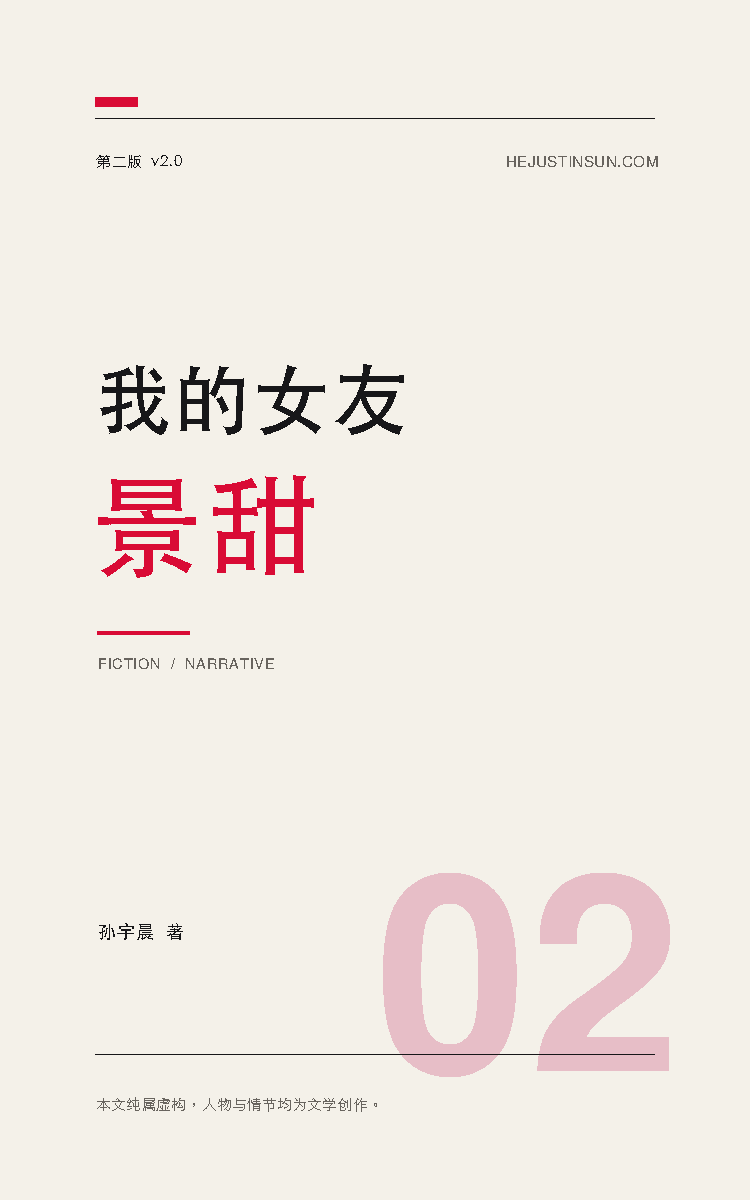
\includepdf[
  pages=1,
  fitpaper=true,
  noautoscale=true,
  pagecommand={\thispagestyle{empty}}
]{../assets/cover.pdf}

\pagenumbering{arabic}
\setcounter{page}{1}
\pagestyle{bodyrunning}
\thispagestyle{bodyopening}
% Opening-page breathing room.
\vspace*{70.817pt}

\StoryParagraph{3}{The weight of one egg: three point five micrograms.}

\StoryParagraph{3}{The weight of fifty million dollars in cash: two point five tons.}

\StoryParagraph{3}{What Jing Tian asked me for, on the phone from the Montage Laguna Beach, was the latter. The collateral was the former.}

\StoryParagraph{3}{She had gone there for the egg retrieval. The surrogate child was due in 2027; if things moved fast, it could still be born in the Year of the Horse. She was the one who had brought it up. Then, at the clinic, she said: no fifty million, no retrieval.}

\UnprintedPause

\StoryParagraph{0}{The Montage Laguna Beach sits on a bluff above the Pacific. We took the whole floor, thirty days, one million dollars, for her privacy. She stayed eight days and left.}

\StoryParagraph{0}{For the remaining twenty-two days, the hotel's housekeepers went up as usual. My assistant told me; she ran into it once, returning the keys: a Mexican woman pushing a cart, going room by room, changing the towels, wiping the counters, tucking in the corners of the sheets, backing out and pulling the door shut. The whole floor took two hours.}

\StoryParagraph{0}{My assistant asked her why she still did the rooms when no one was staying in them.}

\StoryParagraph{0}{She said, the register says occupied.}

\StoryParagraph{0}{A Versailles that had lost its queen.}

\StoryParagraph{0}{It came to me suddenly: Jing Tian liked this. Jing Tian liked a place standing empty because of her. Nothing happens.}

\StoryParagraph{3}{Standing empty along with the Montage Laguna Beach: a Gulfstream G700 parked awkwardly at Van Nuys, the crew reporting for duty every day as usual.}

\StoryParagraph{3}{On the eighth day she made that call. After that, no one saw her again.}

\NarrativeBreak

\StoryParagraph{0}{In 2007, someone was already burning money for her. That was the year I entered Peking University.}

\StoryParagraph{3}{The one burning money, of course, was not me.}

\StoryParagraph{3}{A QQ window popped up. She was the face of the campaign. On that old Lenovo-IBM machine, the resolution was a blur. I saved the picture.}

\StoryParagraph{3}{From my Peking University dorm, where the rent was a thousand yuan a year, I got online, found her on Xiaonei (the Chinese Facebook clone), and sent a friend request. Xiaonei required a message. I wrote and deleted, deleted and wrote, for about forty minutes, and in the end sent one line: “Hello.”}

\StoryParagraph{3}{She never accepted.}

\StoryParagraph{3}{She may never have used Xiaonei at all.}

\StoryParagraph{3}{In all the years after, whatever I was doing, I was asking one question: at what point would she accept. At the first billion I wondered. At ten billion I wondered.}

\StoryParagraph{3}{Then I stopped wondering. Renren had long since gone under.}

\StoryParagraph{3}{I never sent a second request.}

\StoryParagraph{3}{In 2011, Beijing was cold. I bought a down jacket, a hundred and fifty yuan. I remember the price because I hesitated for three days.}

\StoryParagraph{3}{That same year she made The Warring States, a film that cost a hundred and fifty million yuan. Sun Honglei, Francis Ng, Kim Hee-sun, Kiichi Nakai, Jiang Wu were brought in as backdrop, like the Montage Laguna Beach and the Gulfstream G700 nineteen years later. They did not know why they were there; but they had come, and something ought to happen. Nothing happened.}

\StoryParagraph{3}{Then came The Great Wall, a hundred and fifty million U.S. dollars. Zhang Yimou, Andy Lau, Matt Damon. Then Jackie Chan. The roster of the Jing Tian universe grew longer and longer.}

\StoryParagraph{3}{By then I was in America, studying, starting companies, busier and busier. The one thing that never changed: every time I switched devices, however much trouble it was, I carried that QQ picture over.}

\StoryParagraph{3}{Nineteen years later, my name was added to the roster.}

\NarrativeBreak

\StoryParagraph{3}{We met for the first time at the Rosewood. I had always assumed that the day I saw her I would be nervous.}

\StoryParagraph{3}{I was not.}

\StoryParagraph{3}{She was thinner than her pictures, dressed carelessly, leaning back on the sofa. I looked at her and suddenly could not remember what it was I had been waiting for.}

\StoryParagraph{3}{I took her to see Cattelan's banana. She looked at it a long time and asked me, how much is this.}

\StoryParagraph{3}{Six point two million dollars.}

\StoryParagraph{3}{She said, then what happens when it rots.}

\StoryParagraph{3}{I fell silent. She said, forget it, let's go see a movie.}

\StoryParagraph{3}{I said okay.}

\StoryParagraph{3}{She said there could be no one in the theater but the two of us.}

\StoryParagraph{3}{I said okay.}

\StoryParagraph{3}{I went out and made a phone call. When I came back she was still standing in front of the banana.}

\StoryParagraph{3}{The movie was Zootopia 2.}

\StoryParagraph{3}{A screening room with two people in it. The usual occasion for that is a private screening for the censors.}

\StoryParagraph{3}{I had my assistant buy every seat in the cinema.}

\StoryParagraph{3}{I had read the articles denouncing fake box office numbers — tickets sold out, two people in the seats. Now I understood. Maybe it was not entirely about the box office.}

\StoryParagraph{3}{Buying out the seats was easy. The trouble was the tickets already sold. My assistant and the bodyguards went to the entrance ahead of time, and when a ticket-holder showed up, handed over cash.}

\StoryParagraph{3}{A couple came with their child; the child was already at the door, holding the popcorn up high.}

\StoryParagraph{3}{My assistant handed over a stack of bills. The child did not understand why they could not go in. The adults took the money, said thank you, asked nothing, and left.}

\StoryParagraph{3}{Twenty-six people took the money that day.}

\StoryParagraph{3}{Afterward she changed her WeChat avatar to Officer Judy Hopps.}

\StoryParagraph{3}{That night I was rubbing her tits with my hand, and she pushed me away.}

\StoryParagraph{3}{I thought she did not want it. I drew my hand back and started to think of something to say.}

\StoryParagraph{3}{She said nothing. She sat up, dug a small pouch out of her bag, unzipped it. Inside was a row of things, like a very small set of tools.}

\StoryParagraph{3}{She said, your nails jab into me, it hurts.}

\StoryParagraph{3}{I took a look. All my life I had trimmed them with clippers, two quick cuts, sharp at the edges. I had never noticed.}

\StoryParagraph{3}{She said, come here.}

\StoryParagraph{3}{She laid my hand on her thigh and filed the nails one by one.}

\StoryParagraph{3}{First the coarse side; when that was done, the next side, then the next. Every so often she lifted my hand to the light, looked, and went on filing.}

\StoryParagraph{3}{I said, how long does this take.}

\StoryParagraph{3}{She said, until they don't scratch.}

\StoryParagraph{3}{Ten fingers. It took her nearly an hour.}

\StoryParagraph{3}{Along the way she taught me: this side is for shape, this side is for polish, and with the last side you don't rub back and forth, you go in one direction.}

\StoryParagraph{3}{I said okay.}

\StoryParagraph{3}{When she finished she turned my hand over, looked at it, ran a finger across it.}

\StoryParagraph{3}{She said, done.}

\StoryParagraph{3}{Touch me. Anywhere you want.}

\StoryParagraph{3}{In the middle of it she said one thing. She said, if someday I'm gone, no one will ever polish your nails again.}

\StoryParagraph{3}{I smiled a little and said nothing.}

\StoryParagraph{0}{Three months after I met her, I had something put together. Her projects over the years, her partners, her company shareholdings, Jing Guoqing, Tian Xin'ai, all the linked accounts, the apartment rented in Beijing, the one bought in Shanghai, and some other things. It took a week; forty-some pages. There were also the affairs, men and women. I considered that the least important part.}

\StoryParagraph{0}{Some of the things in it she told me about later, and what she told me was not quite what was written. I did not say so.}

\StoryParagraph{0}{Some things she never told me. I did not ask.}

\StoryParagraph{0}{I believed everything she said.}

\StoryParagraph{0}{That document I kept. I have it still.}

\StoryParagraph{3}{But I did not believe one word of it.}

\NarrativeBreak

\StoryParagraph{3}{She said, Hong Kong has too many people, I'll be recognized. Let's go somewhere.}

\StoryParagraph{3}{I said okay.}

\StoryParagraph{3}{She put a finger on the map, on Tenerife.}

\StoryParagraph{3}{I said okay.}

\StoryParagraph{3}{I went out and made a phone call. Only when I came back did I learn that the place lies in the Atlantic off the northwest coast of Africa. The next day at noon, the thirty of us set out; the A330 was waiting at the airport.}

\StoryParagraph{3}{In the bedroom of the plane she asked me, is my name pretty.}

\StoryParagraph{3}{I said it was pretty.}

\StoryParagraph{3}{She said, it's my father's surname and my mother's surname joined together, isn't that a coincidence.}

\StoryParagraph{3}{I said I had memorized it on the first day.}

\StoryParagraph{3}{She held me and said, don't call me Jing Tian anymore. Call me Mama.}

\StoryParagraph{3}{Okay, Mama.}

\StoryParagraph{3}{After we landed the captain came to tell me: boss, at first the island wouldn't clear us to land. They had never seen a private jet this big.}

\StoryParagraph{3}{The rule on the island was the same: no one nearby. The assistants went to arrange it. No one asked why. This time I did not ask how many people.}

\StoryParagraph{3}{The Ritz-Carlton faced the Atlantic, and the windows were too big. She could not sleep with a sliver of light. The assistants taped up the whole room with black tape — outside bright as noon, inside dark as a cell. The tape peeled in the sun and had to be redone every day.}

\StoryParagraph{3}{There were eleven assistants in all; they arrived at six-thirty in the morning and left after we slept. Two girls did the taping, one on the window frames, one on the indicator lights of the air conditioner and the outlets, and when they finished they checked it three times over. They bought thirty rolls of tape, then twenty more. They discovered that tape laid after three in the afternoon peeled soonest, because that was when the glass was hottest, so they switched to taping in the morning. No one taught them this. They worked it out themselves. They discussed it with each other, like a craft.}

\StoryParagraph{3}{She knew the two girls' names. I did not.}

\StoryParagraph{3}{We stopped by the road in Teide National Park to watch the sunset. The assistants carried roses down from the cars and opened champagne.}

\StoryParagraph{3}{Mama looked at the sea of clouds and said, beautiful. But not as good as the sunset at Delingha, in Qinghai.}

\StoryParagraph{3}{I am from Qinghai.}

\StoryParagraph{3}{I did not say so.}

\StoryParagraph{3}{At night we watched the stars from the summit, cold even in padded coats.}

\StoryParagraph{3}{Mama said, make a wish.}

\StoryParagraph{3}{I asked, what did you wish for.}

\StoryParagraph{3}{Mama said, I'm not telling.}

\StoryParagraph{3}{Mama said, it's too beautiful. But it's just too cold. Let's go to the Maldives, all right?}

\StoryParagraph{3}{I said, all right.}

\StoryParagraph{3}{Tenerife was fifteen below; the Maldives, twenty-seven degrees. Nine thousand five hundred kilometers in a straight line, eleven hours in the air. But the airport in the Maldives was too small; midway we would have to trade the wide-body for a small plane.}

\StoryParagraph{3}{Mama said, the small plane is so loud. Big planes are better.}

\StoryParagraph{3}{In the bedroom of the plane to the Maldives, Mama told me her wish: a child, with me. It had to be a surrogate.}

\StoryParagraph{3}{I never asked why. I assumed she was afraid of the pain.}

\StoryParagraph{3}{Midway Mama sat up suddenly, hunting for her phone, connected to Starlink, and said, oh no.}

\StoryParagraph{3}{I asked what was wrong.}

\StoryParagraph{3}{She said, someone is threatening me. He's been asking for three days and I haven't answered.}

\StoryParagraph{3}{I said how much.}

\StoryParagraph{3}{She said, you stay out of it.}

\StoryParagraph{3}{She typed for a long time, deleting and rewriting, rewriting and deleting. When she finished she laid the phone face-down on her leg, then after a while turned it over to look.}

\StoryParagraph{3}{I asked who it was.}

\StoryParagraph{0}{She said, someone who used to be with me. Finance. Went to prison. Took the fall.}

\StoryParagraph{3}{Out now, nowhere left to go, and he had to come find me.}

\StoryParagraph{3}{I said, just call the police and have him taken.}

\StoryParagraph{3}{She gave me a look. You don't understand.}

\StoryParagraph{3}{I said did you pay.}

\StoryParagraph{3}{She said she paid.}

\StoryParagraph{3}{How much.}

\StoryParagraph{3}{Eighty thousand.}

\StoryParagraph{3}{I said, and that took three days of thinking.}

\StoryParagraph{3}{She said nothing.}

\StoryParagraph{3}{For the rest of that day she hardly spoke. She fell asleep only after we landed.}

\StoryParagraph{0}{The first thing to reach Soneva Jani was Mama's suitcase. Thirty people's luggage would not fit in the small planes; it went in three. Mama had one suitcase, and it flew alone. She said it was not to be put with anyone else's.}

\StoryParagraph{0}{Soneva Jani is famous for no news, no shoes. Mama relaxed.}

\StoryParagraph{3}{Hotel butlers, bodyguards, assistants: twenty-six people assigned, plus two drone operators trailing at a distance. The assistants started taping again — the air-conditioner light, the outlet lights, over and over.}

\StoryParagraph{0}{At night we traded our exes like passwords, like a dynasty collating its era names. Mama would tolerate no discrepancy. But Mama had one forbidden word: the athlete was not to be mentioned.}

\StoryParagraph{0}{I did not mention him, though I knew the tattoo on Mama's back had been done for the athlete.}

\StoryParagraph{3}{Probably it was too big to remove.}

\StoryParagraph{0}{She said, we're family now. My parents went to no small trouble raising me. You have to pay the bride price.}

\StoryParagraph{0}{I said okay.}

\StoryParagraph{0}{She gave two names, Jing Guoqing and Tian Xin'ai, and two account numbers.}

\StoryParagraph{0}{Thirty million, renminbi.}

\StoryParagraph{0}{I transferred it. Those two names — the first place I ever saw them was in those forty-some pages.}

\StoryParagraph{3}{A while later she held out her phone for me to see. Tian Xin'ai had replied with one word: Received.}

\StoryParagraph{0}{Once Mama said, do you know what I'm thinking when I ask you for these things.}

\StoryParagraph{0}{I said what.}

\StoryParagraph{0}{She said, I'm thinking: will there ever be a time you say no.}

\StoryParagraph{0}{I said there wouldn't.}

\StoryParagraph{0}{She said, then it's no fun.}

\StoryParagraph{3}{I thought: was there anything I could not do?}

\StoryParagraph{0}{In the dead hours I was fiddling with the 2007 QQ picture, moving it onto a new device. Mama leaned her head in: so you keep another woman's photo behind my back. Who is this.}

\StoryParagraph{0}{I fell silent. I said nothing.}

\StoryParagraph{0}{She found the picture too blurry to make out and went off to do something else.}

\StoryParagraph{0}{That night I deleted the picture.}

\StoryParagraph{3}{The next day I recovered it from an old phone.}

\StoryParagraph{0}{Mama scrolled her phone without end too. I asked what she was reading.}

\StoryParagraph{0}{She said, nothing. Just the usual filth of fighting over top billing.}

\StoryParagraph{0}{Fighting over top billing: a production can have only one star listed first. Between the male lead and the female lead, too, only one name comes first.}

\StoryParagraph{0}{I said, how boring.}

\StoryParagraph{0}{She said, yes. What's harder: sometimes there's a set couple. Forty, fifty days into a production, playing opposite the same man, making love at night and still fighting over top billing by day.}

\StoryParagraph{0}{I said, that's against human nature.}

\StoryParagraph{0}{She said, yes.}

\StoryParagraph{0}{But once the film wraps, however many times they made love, it's as if none of it ever happened.}

\StoryParagraph{3}{Then she read for another half hour.}

\StoryParagraph{0}{January 2, 2026. Soneva Jani, the new year. I proposed to Mama.}

\StoryParagraph{0}{I had decided on the morning of January 1. The ring was in Hong Kong. There was nowhere on the island to buy one, so an assistant took the seaplane to Malé and came back in the afternoon with the ring in one of the hotel's envelopes.}

\StoryParagraph{0}{Mama said, the diamond is too small.}

\StoryParagraph{0}{Mama said, it's fine. Get me a bigger one later.}

\StoryParagraph{0}{Also — can you come to Beijing?}

\StoryParagraph{0}{I fell silent.}

\StoryParagraph{0}{She thought I did not want to go.}

\StoryParagraph{0}{Mama said, why are you so good to me.}

\StoryParagraph{0}{I said because I like you.}

\StoryParagraph{0}{She said, and were you like this with the others before.}

\StoryParagraph{0}{I said no.}

\StoryParagraph{3}{She smiled a little and said nothing.}

\StoryParagraph{0}{One morning I woke early and she was not in bed.}

\StoryParagraph{0}{I went out. She was sitting on the deck, facing the sea, and the whole sea was black. No lights on; not light yet.}

\StoryParagraph{0}{I asked why she was up so early.}

\StoryParagraph{0}{She said, I'm counting days.}

\StoryParagraph{0}{I said counting what.}

\StoryParagraph{0}{She said, go back to sleep.}

\StoryParagraph{0}{I sat beside her a while, not knowing what to say. Then I went back to sleep.}

\StoryParagraph{3}{When I woke again her makeup was already done.}

\StoryParagraph{0}{Fourteen days in the Maldives and not one person recognized her.}

\StoryParagraph{0}{On the thirteenth night, in the restaurant, she took off her sunglasses. A while later the hat came off too, and she set it on the table. She sat that way through the whole meal. The next table was an old German couple; the waiter was Sri Lankan. No one gave her a second look.}

\StoryParagraph{0}{When the meal was over she put the hat back on.}

\StoryParagraph{0}{Mama said, let's go back.}

\StoryParagraph{0}{I said, but we haven't stayed long enough yet, have we.}

\StoryParagraph{3}{She said, it's too quiet.}

\UnprintedPause

\StoryParagraph{0}{Back in Hong Kong, Mama met my parents.}

\StoryParagraph{0}{That night she said the family had to prepare for the two households to meet, and for the wedding; smooth the way as generously as possible. Jing Guoqing and Tian Xin'ai again.}

\StoryParagraph{0}{I did not ask why.}

\StoryParagraph{0}{I said each card has a limit of one million a day.}

\StoryParagraph{0}{Mama said too slow.}

\StoryParagraph{0}{Transfer from five.}

\StoryParagraph{0}{Five cards, two accounts, in rotation. At the third card I hesitated. I finished the transfers anyway.}

\StoryParagraph{3}{Mama said, this is so inefficient.}

\StoryParagraph{0}{I said, for New Year let's bring both our parents to Hong Kong and spend it together.}

\StoryParagraph{0}{Mama said, this year is already set for Hainan. Next year.}

\StoryParagraph{0}{At Spring Festival the fireworks went off over Victoria Harbour and a million people came. She was not among them.}

\StoryParagraph{0}{At three in the morning I took my parents home.}

\StoryParagraph{0}{The roads were empty. At the red light not one car was waiting. I stopped anyway.}

\StoryParagraph{0}{Mama said no meeting for now — she was about to go to Los Angeles for the retrieval. Things in hand had to be closed out first.}

\StoryParagraph{0}{Mama asked again, can you come to Beijing?}

\StoryParagraph{0}{I fell silent.}

\StoryParagraph{3}{She did not say what was in Beijing. I did not ask.}

\StoryParagraph{0}{Mama said, there must be an apartment in Hong Kong, in her name.}

\StoryParagraph{0}{I said, all right.}

\StoryParagraph{3}{We did not meet on Valentine's Day either.}

\StoryParagraph{0}{Once on the phone she said, they took eight tubes of blood this morning.}

\StoryParagraph{0}{I said that many.}

\StoryParagraph{0}{She said it was all right.}

\StoryParagraph{0}{I said, that's hard on you.}

\StoryParagraph{0}{Then we talked about other things.}

\StoryParagraph{0}{Only later did I learn that blood like that is drawn fasting, on the second or third day of the cycle; the date cannot slip. That morning she must have left around six, a Beijing winter, dark before dawn. The tests kept multiplying. I knew about it because a new item had appeared in the assistant's monthly payment summary. The first time was last year, a small amount, a few thousand yuan. After that it came every month, sometimes two or three entries. I approved them fast. Amounts like that I don't read line by line. Only later did I learn what they were: blood draws, the six-hormone panel, ultrasounds, AMH. To see how much reserve she had left, how many could be retrieved, whether it was worth going on.}

\StoryParagraph{0}{All of it was done in Beijing.}

\StoryParagraph{3}{I don't know which hospital. I don't know whether she went alone or someone went with her.}

\StoryParagraph{0}{On February 25 she landed in Hong Kong.}

\StoryParagraph{0}{She said she would not go to Los Angeles unless she saw the Hong Kong apartment first.}

\StoryParagraph{0}{I sent her the dozen or so apartments we had looked at over the past half year. She found them all ugly. I had never set foot in a single one; the assistant had spent six months choosing them one by one, the assistant forwarded them to me, I forwarded them to her. One was on the Mid-Levels, and in the video you could see Victoria Harbour; it was shot at dusk. For an instant the camera wobbled and caught, on the wall, the shadow of the person filming. I looked at that shadow and thought: who is this, how far did he walk today, how many apartments did he see, does he know who this one is for.}

\StoryParagraph{3}{Time was too short. She boarded the G700 for Los Angeles anyway, and on February 28 she reached the Montage Laguna Beach.}

\NarrativeBreak

\StoryParagraph{0}{On the eighth day Mama called. It was afternoon where she was, the small hours where I was.}

\StoryParagraph{0}{She said, fifty million. Dollars.}

\StoryParagraph{0}{I said, let me think.}

\StoryParagraph{0}{She said nothing. I could hear the sea on her end.}

\StoryParagraph{0}{After a while she said, okay.}

\StoryParagraph{0}{She hung up.}

\StoryParagraph{3}{In all the time I had known her, I had never once said “let me think” to her.}

\StoryParagraph{0}{I ran every cash asset through Claude Code, reading the APIs, and the conclusion was that it would not affect me at all. I checked it again. I typed the question into Claude Code. Claude said, do not give her the fifty million dollars.}

\StoryParagraph{3}{I asked, does she not love me anymore?}

\StoryParagraph{3}{Claude said, as for love, I do not care about it, and I do not understand it. But you cannot give her the fifty million dollars.}

\StoryParagraph{3}{I had never refused her. Not out of generosity — out of fear. Fear of what the next second's answer would be.}

\StoryParagraph{0}{And now someone had said it for me.}

\StoryParagraph{0}{I stared at that line for a long time. What made my skin crawl was not that it was smart. It was that Claude had not hesitated at all.}

\StoryParagraph{0}{It was not torn.}

\StoryParagraph{0}{I thought at the time, this must be something higher. A human cannot do this.}

\StoryParagraph{3}{Does she not love me anymore.}

\StoryParagraph{3}{The next day she called back.}

\StoryParagraph{3}{Mama said, the sea is big.}

\StoryParagraph{3}{I said is it.}

\StoryParagraph{3}{She said, this floor is too big, there's an echo. In the morning the cleaners come, and I hide in the bathroom until they leave.}

\StoryParagraph{3}{I said I could have them not come.}

\StoryParagraph{3}{She said no need.}

\StoryParagraph{3}{She said, the clinic asked me when the child's father is coming.}

\StoryParagraph{3}{I said I could send someone.}

\StoryParagraph{3}{She said, no need.}

\StoryParagraph{3}{Then she said, have you thought it over.}

\StoryParagraph{3}{I said nothing. I was not thinking. I was not thinking anything at all. On her end of the line there was the sea; on mine, Victoria Harbour; no one spoke on either end. I counted. Eleven seconds.}

\StoryParagraph{3}{Jing Tian said, fine.}

\StoryParagraph{3}{Jing Tian said, I see.}

\StoryParagraph{3}{She hung up.}

\StoryParagraph{3}{Afterward I went back over it countless times: those two days, what else she had said besides the fifty million. The sea is big. This floor is too big. She hid in the bathroom. That was all, and I remember all of it, word for word. What I cannot recall is her voice — when she said “I see,” what the tone was.}

\StoryParagraph{0}{I could not recall it. After a while I stopped trying.}

\StoryParagraph{0}{I set the phone on the nightstand, screen down. Then I did something I still cannot explain: I put my hand on my chest and counted.}

\StoryParagraph{0}{The heartbeat was steady.}

\StoryParagraph{0}{I counted again. Still steady. Sixty-some a minute, no different from any other day. I sat there with my hand pressed to my chest, like a doctor examining someone else.}

\StoryParagraph{3}{I thought: so that's how it is.}

\StoryParagraph{0}{I did nothing for the rest of that day. I stayed in the room from dark to dawn, watching Victoria Harbour go from blue to grey to black. At six in the morning the towers of the financial district across the harbour began to light up, one by one. At some point an assistant knocked to ask about dinner. I said no need.}

\StoryParagraph{3}{I did not cry. I kept waiting to cry.}

\NarrativeBreak

\StoryParagraph{0}{Later the assistant settled the accounts with me, and one item was compensation to the hotel on Tenerife. After we left, the tape had gone up for several more days; no one had told the girls to stop. The hotel said it had been taped too long, too many times; the adhesive marks on the frames would not come off, and the whole pane had to be replaced.}

\StoryParagraph{0}{I said approved.}

\StoryParagraph{3}{That pane of glass faces the Atlantic.}

\StoryParagraph{0}{On the bill, the line for jet fuel came to more than the whole floor at the Montage. I asked about it. The assistant said, the A330 is designed for two hundred people and we were only thirty — too light, the trim was off for takeoff. So each time they added fuel until the plane was heavy enough. And at the destination the extra could not stay aboard; it had to be dumped.}

\StoryParagraph{0}{I said, every time?}

\StoryParagraph{3}{He said, every time.}

\StoryParagraph{0}{And there was a box the Los Angeles clinic sent back. Eight days of stimulation shots, the refrigerated kind, not one opened.}

\StoryParagraph{3}{And the surrogacy agency's deposit, two hundred thousand dollars, nonrefundable. The surrogate had been booked in January. A Californian, thirty-four, two children of her own. Her photograph is in the file. I have not looked at it. She was ready in January.}

\StoryParagraph{3}{After Jing Tian left, I took out the 2007 picture and looked at it once. Nineteen years; the devices' pixels climbed higher and higher, and this picture seemed to sink lower and lower, the face all blur. I zoomed in and looked a long time, trying to find where she differed from the woman who came later. I could not find one place. Because the picture had never been clear to begin with.}

\StoryParagraph{0}{One day I cut my nails with the clippers, and when I was done I touched them. Sharp.}

\StoryParagraph{0}{I remembered the thing in the drawer, the one she left.}

\StoryParagraph{0}{I took it out and gave the nails a couple of strokes. Wrong. She had said to go in one direction, and I had forgotten which direction.}

\StoryParagraph{0}{I put it back.}

\StoryParagraph{3}{My nails still scratch.}

\StoryParagraph{0}{One morning my phone popped up a reminder, one the assistant had set last year while laying out the calendar: three months before the due date, prepare the room.}

\StoryParagraph{3}{I swiped it away.}

\StoryParagraph{0}{Since she left, I have been turning over one question.}

\StoryParagraph{0}{If I had given it that day, would she have stayed.}

\StoryParagraph{0}{I thought about it a long time.}

\StoryParagraph{3}{In the end I took that document out and read it again. Forty-some pages.}

\StoryParagraph{0}{Then I remembered the night of Spring Festival, looking down from the rooftop at the fireworks over Victoria Harbour.}

\StoryParagraph{0}{A million people came in like a tide; the fireworks ended; a million people went out.}

\StoryParagraph{0}{A million people.}

\StoryParagraph{0}{It is like this every year.}

\StoryParagraph{0}{Hong Kong at three in the morning,}

\StoryParagraph{3}{Nothing happened.}

\end{document}
